
%\documentclass[twocolumn]{article}
\documentclass{article}

\usepackage{graphicx}
\usepackage{fullpage}

\begin{document}
\title{WaveScript Benchmarks Perfomance Report}
\maketitle
\date

\subsubsection*{Machine information:}
\input{machineinfo.tex}

\subsubsection*{WaveScript SVN:}
\input{wssvn.tex}

\subsubsection*{WaveScope Engine SVN:}
(omitted for now) %\input{enginesvn.tex}

%% ================================================================================ %%
\section{Microbenchmarks}
%% ================================================================================ %%

This section reports various microbenchmarks that stress the
implementation of particular language constructs or data types.
%Figure \ref{micro} contains execution time results.

%\begin{figure}
\begin{center}
\includegraphics[width=0.9\hsize]{microbench/microbench1.pdf}
\end{center}
%\caption{Microbenchmarks.}\label{micro}
%\end{figure}

\subsubsection*{Per-stream-element overheads}
One thing that you can see, is that currently (2007.10) the
C++/XStream engine has a high per-tuple (that is, per-element) on the communication channels
relative to the ML backend.  The {\tt just\_timer} test stresses this,
doing nothing but passing a large number of unit tuples.

Focusing on scheduling overheads a bit more, we turn to the following
data passing microbenchmarks.  These do nothing but generate a stream
of numbers, and then add up windows of those numbers.  We vary the
window size in the following graphs.  The numbers are passed either
one at a time (``raw''), or in bulk using arrays or lists.

\begin{center}
\hbox{
\includegraphics[width=0.33\hsize]{microbench/datapass10.pdf}
\includegraphics[width=0.33\hsize]{microbench/datapass100.pdf}
\includegraphics[width=0.33\hsize]{microbench/datapass1000.pdf}
}
\end{center}

Notes:
\begin{itemize}
\item FFT results for Scheme above depend on whether or not it is
  configured to use FFTW, or a native Scheme fourier transform.
\end{itemize}



%% ================================================================================ %%
\section{Language Shootout Benchmarks}
%% ================================================================================ %%

This is where I will accumulate some of the small benchmarks from the
language shootout.  Here are some per-benchmark comments:

\begin{itemize}
\item {\bf fannkuch} - ``pancake flipping''.  This is a translation of the
  gcc version of the benchmark.  Tests indexed access to a small array.
\end{itemize}

%\begin{figure}
\begin{center}
\includegraphics[width=0.6\hsize]{language_shootout/shootout.pdf}
\end{center}
%\caption{Great language shootout.  (Those benchmarks that are implemented.)} \label{shootout}
%\end{figure}



%% ================================================================================ %%
\section{Application Benchmarks}
%% ================================================================================ %%

This section includes performance results on larger programs, namely, our
current applications.  

\subsection{Marmot Application}

We start off by looking at the original, hand-optimized marmot
application that we deployed.  We break it down by phase: the first
three phases of the computation, followed by all three together.

\begin{center}
\includegraphics[width=0.6\hsize]{appbench/MARMOT.pdf}
\end{center}

\subsection{Computer Vision: Background Subtraction}


\begin{center}
\includegraphics[width=0.6\hsize]{appbench/BGSUB.pdf}
\end{center}



%% ================================================================================ %%
\section{Data Representation Profiling}
%% ================================================================================ %%

{\bf This is stale data for now... having sneaky problems with the
datarep Makefile that are hosing regression tests. [2007.11.07]}

This section includes an analysis of the efficiency of different data
representations under different backends.  This should theoretically
be run on different hardware platforms as well (such as the ARM-based ensboxes).

\subsection{Arrays of Arrays}

Arrays of arrays are notable because they cannot generally be
flattened (the inner arrays will always be pointers).  In the future
we may look at tentative flattening based on profiling data.  But
first, here are the times for repeatedly allocating an array of
arrays, and for repeatedly folding the values in an array of arrays.

%\begin{minipage}[t]{.45\textwidth} \hfill \end{minipage}
\begin{center}
\mbox{
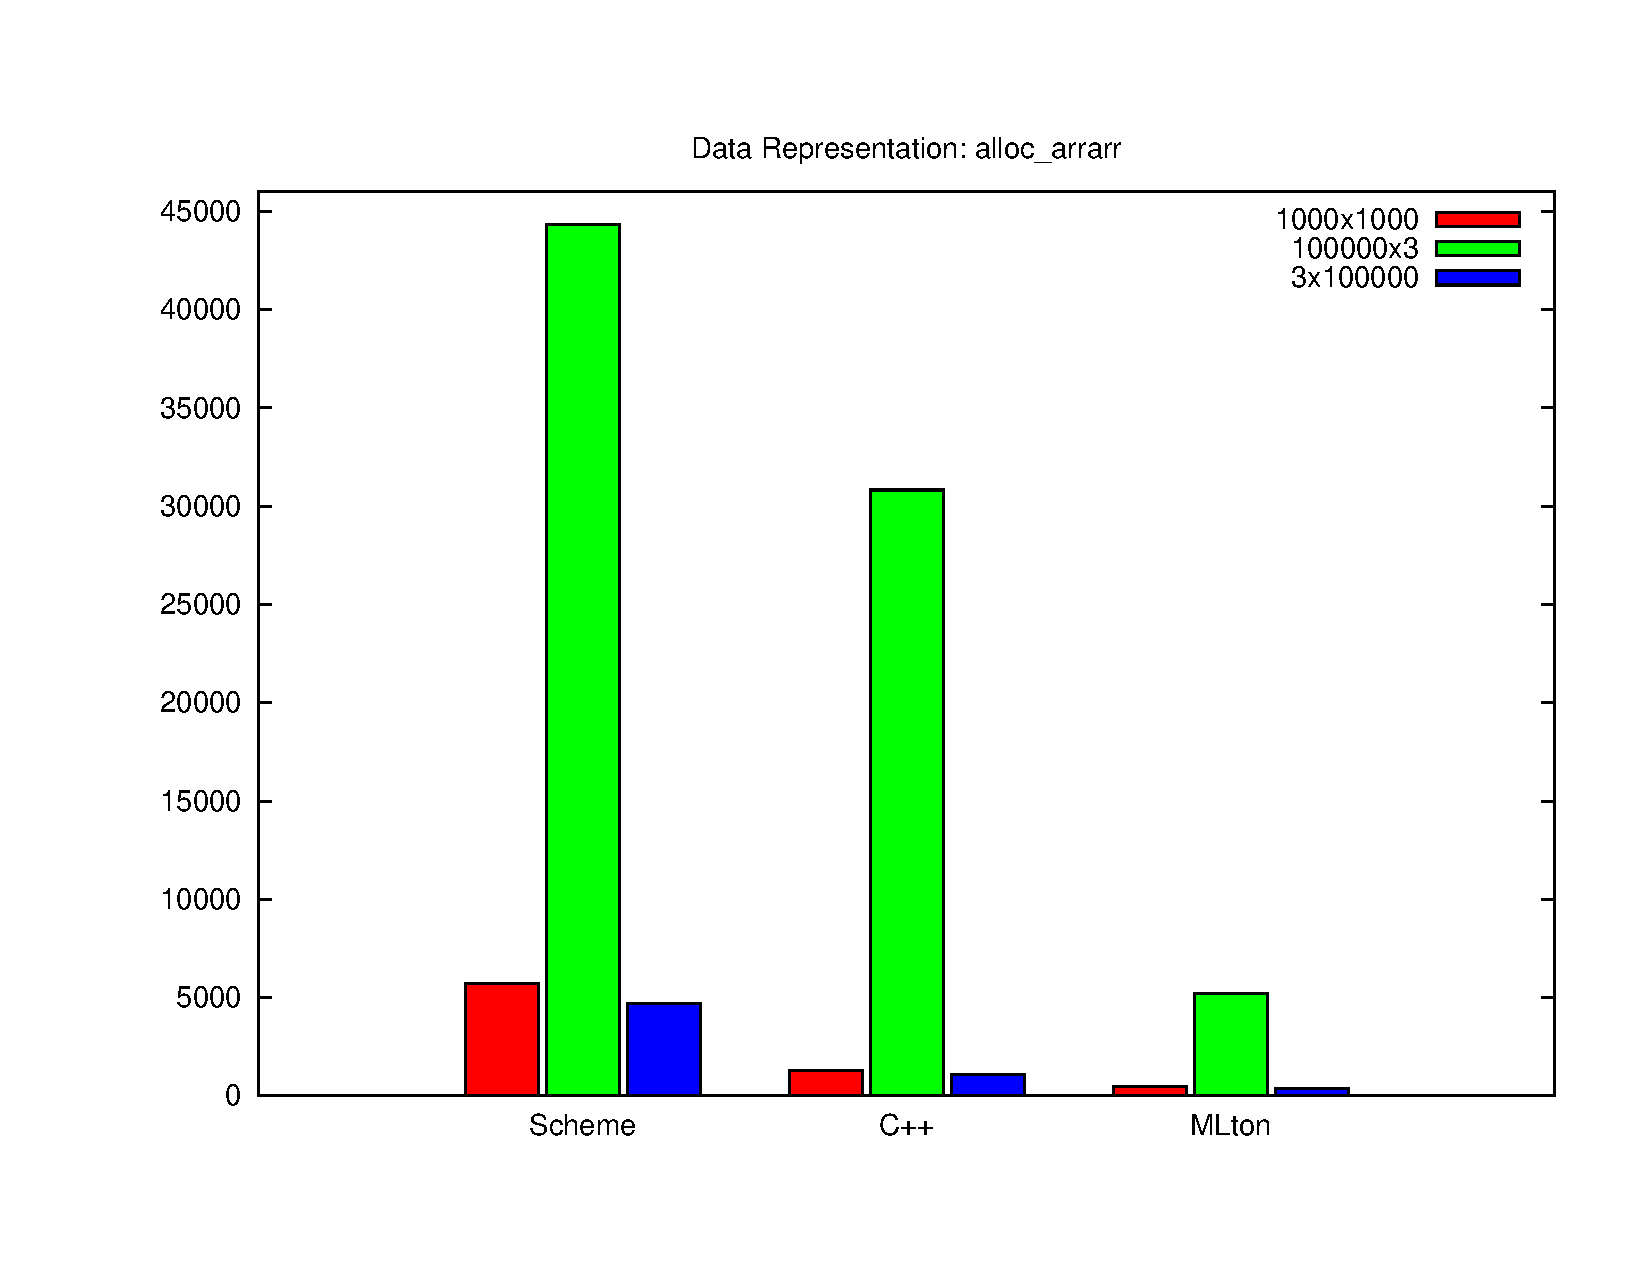
\includegraphics[width=0.48\hsize]{datareps/alloc_arrarr.pdf}
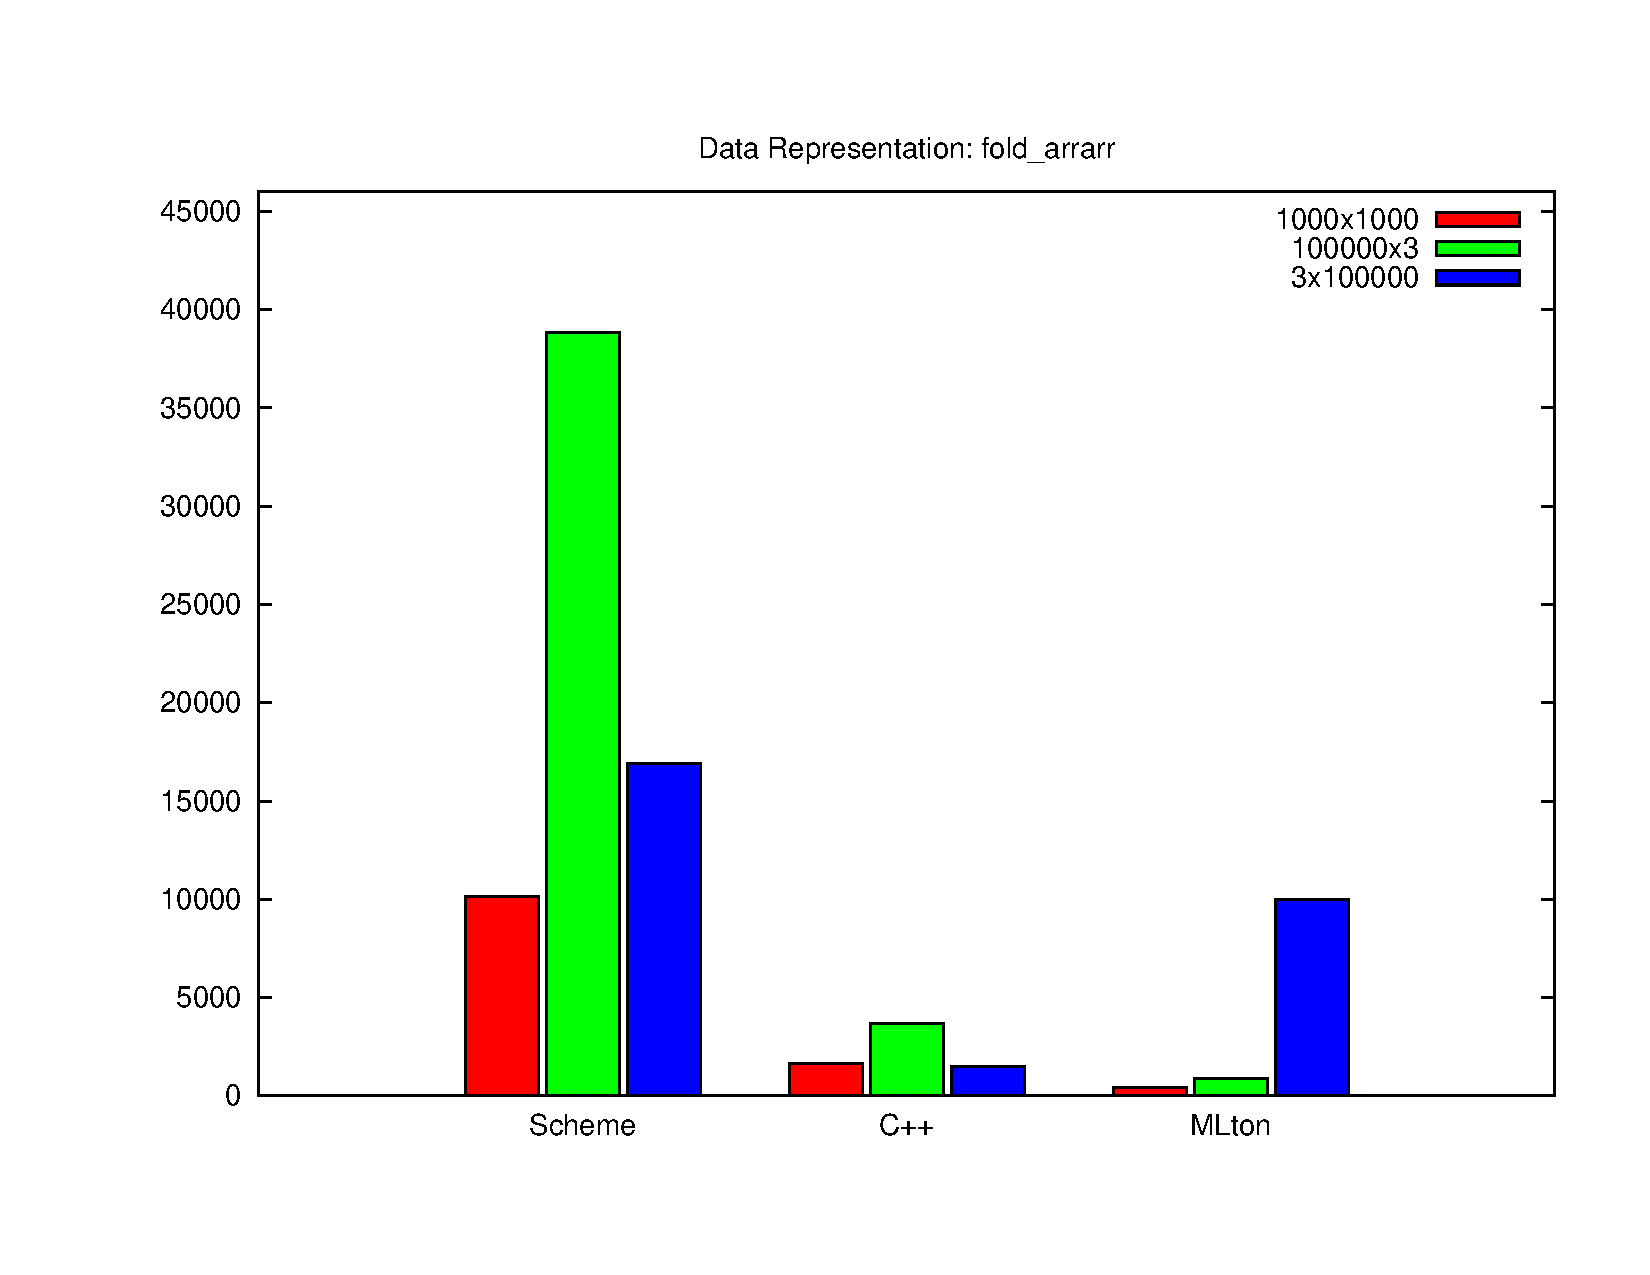
\includegraphics[width=0.48\hsize]{datareps/fold_arrarr.pdf}
}
\end{center}

Next we look at allocating arrays of tuples and vice versa.  We look at
both square sizes and at highly skewed dimensions.  This is limited by
not being able to make tuples very large.
\begin{center}
\mbox{
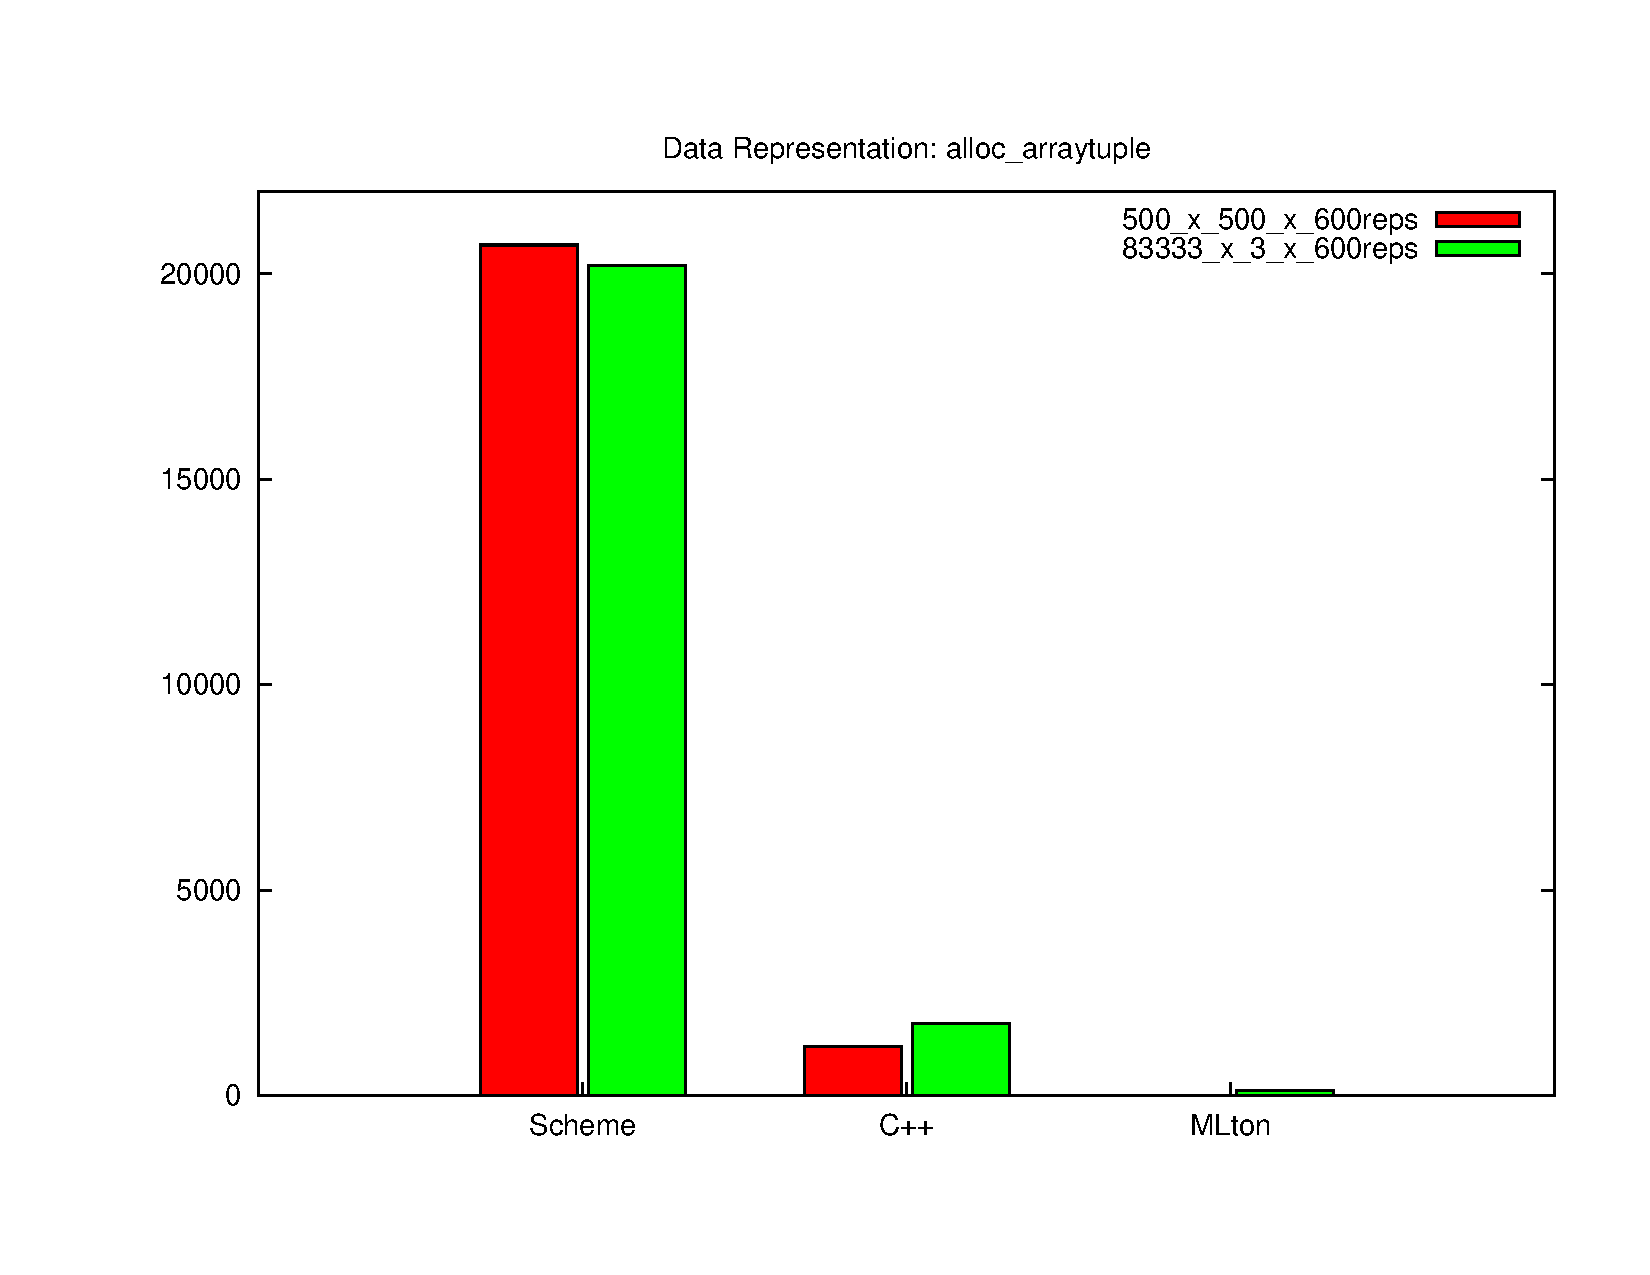
\includegraphics[width=0.48\hsize]{datareps/alloc_arraytuple.pdf}
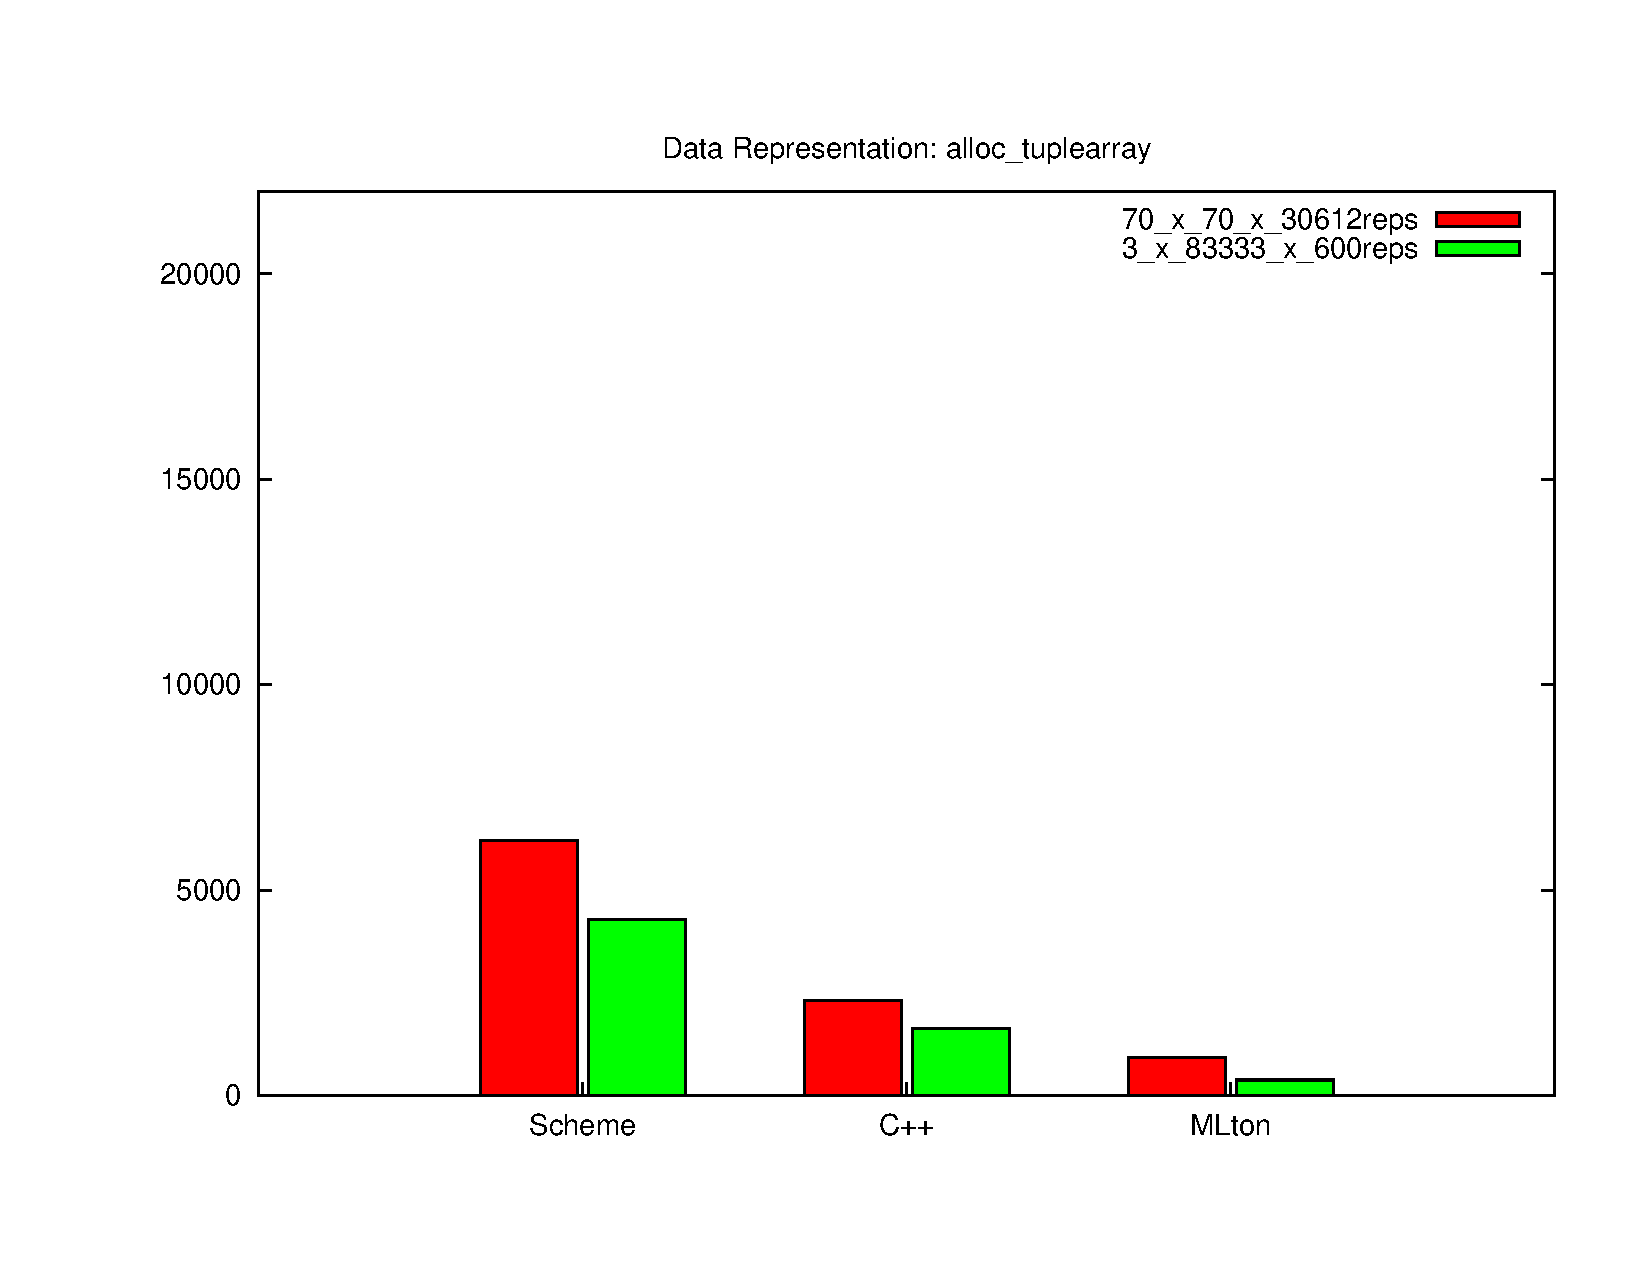
\includegraphics[width=0.48\hsize]{datareps/alloc_tuplearray.pdf}
}
\end{center}

Then we do examine folding over arrays of tuples and tuples of arrays.
\begin{center}
\mbox{
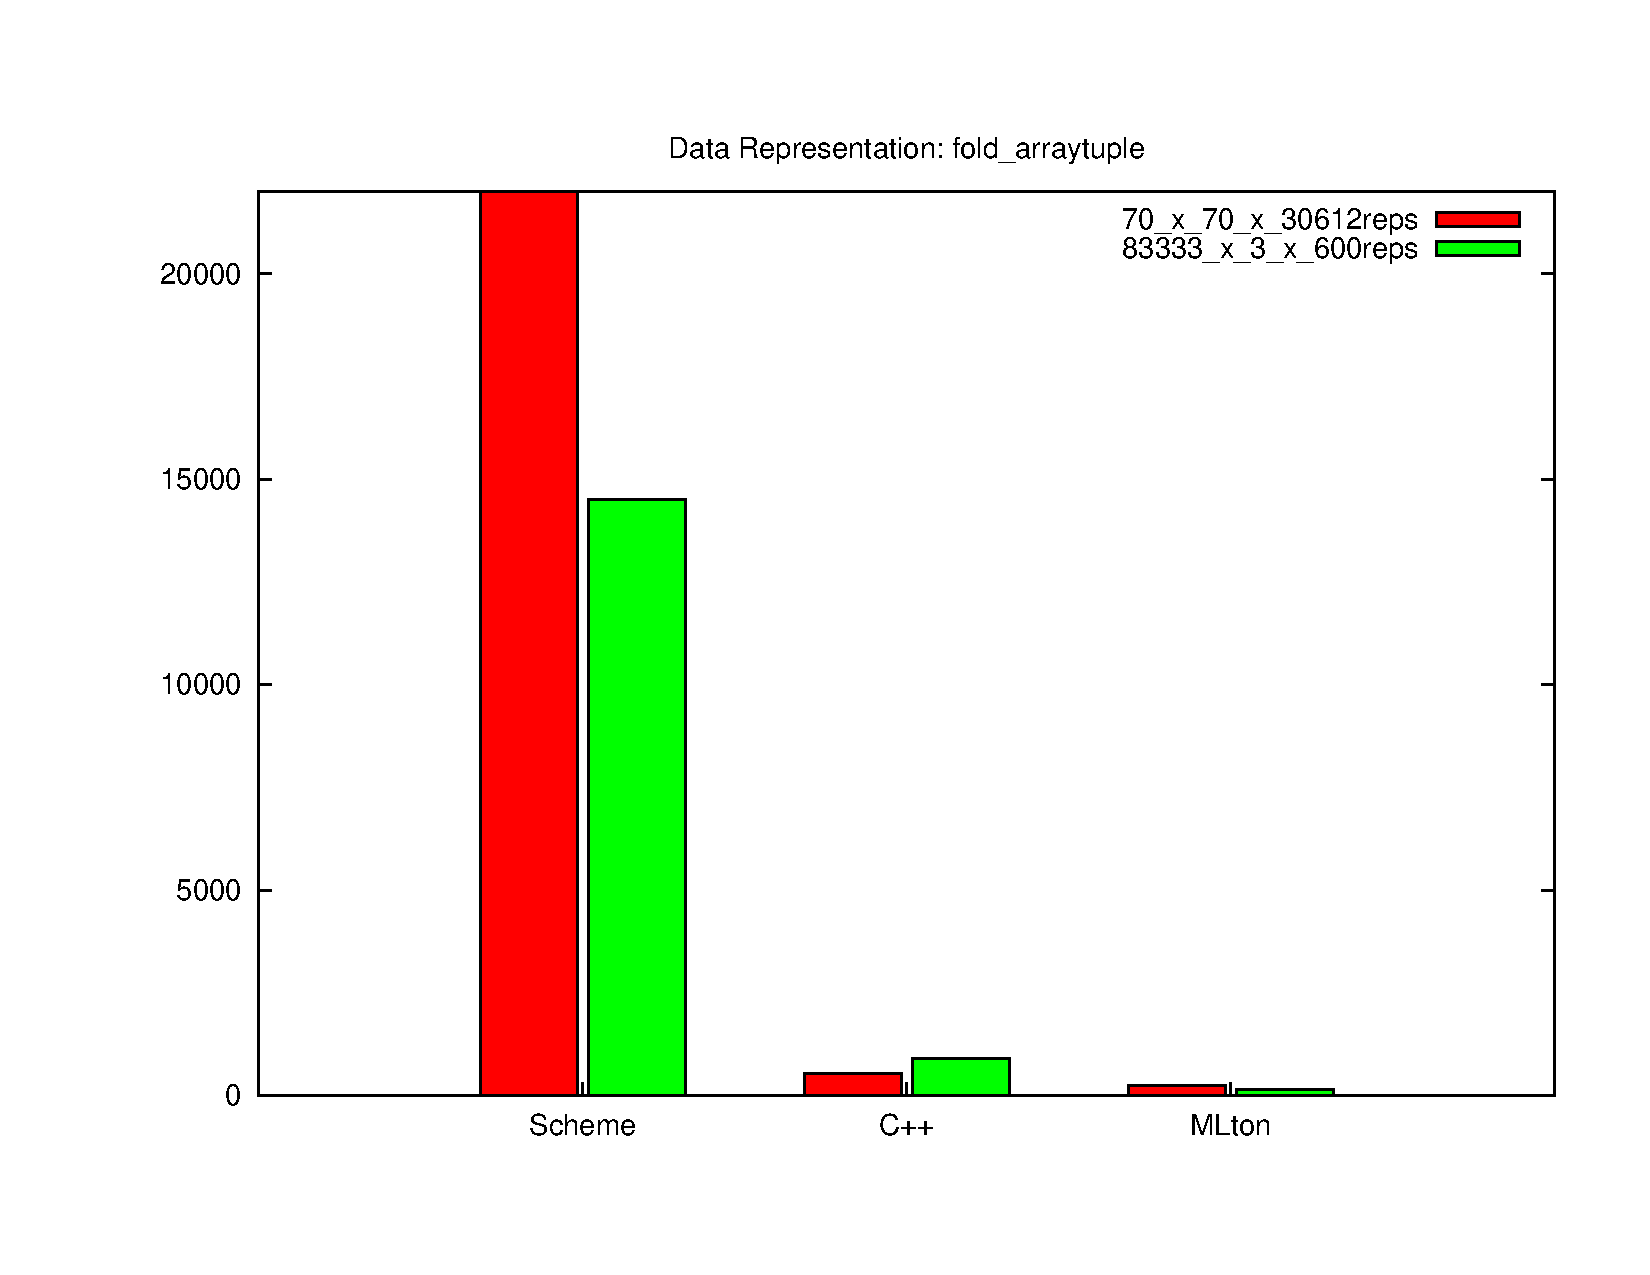
\includegraphics[width=0.48\hsize]{datareps/fold_arraytuple.pdf}
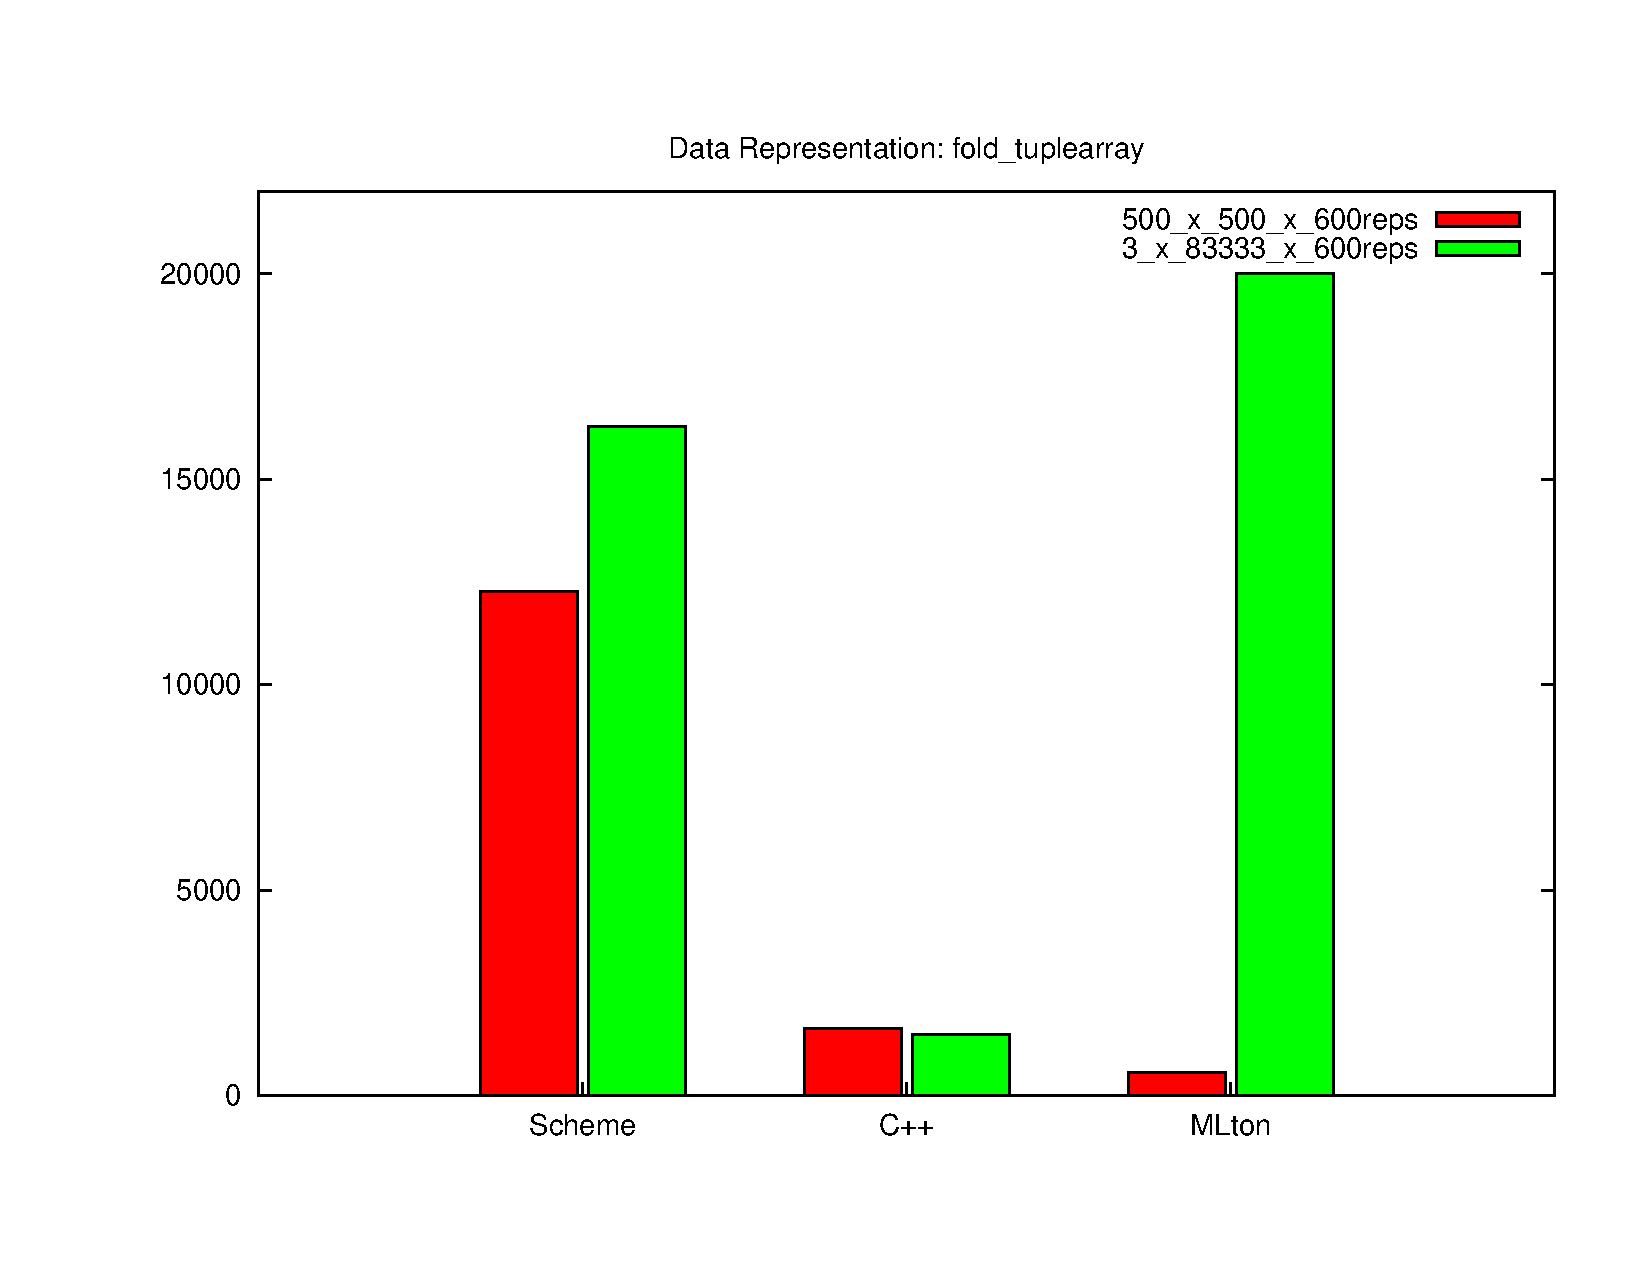
\includegraphics[width=0.48\hsize]{datareps/fold_tuplearray.pdf}
}
\end{center}




%% go3 alloc_arrarr 46000.
%% go3  fold_arrarr 46000.

%% go2 alloc_arraytuple 22000.
%% go2  fold_arraytuple 22000.
%% go2 alloc_tuplearray 22000.
%% go2  fold_tuplearray 22000.




%% ================================================================================ %%
%\pagebreak
\appendix
\section{Appendix: Raw numbers for above graphs}

\subsubsection*{Microbenchmarks}
{\footnotesize
\input{microbench/RESULTS.tex}
}

\subsubsection*{Language Shootout:}
{\footnotesize
\input{language_shootout/RESULTS.tex}}

\subsubsection*{Application Benchmarks:}
{\footnotesize
\input{appbench/RESULTS.tex}}

\section{Appendix: Additional system information}

\subsubsection*{Top results before running benchmarks:}
{
\footnotesize
\input{top_before.tex}
}
\subsubsection*{Top results {\em after} running benchmarks:}
{
\footnotesize
\input{top_after.tex}
}

\end{document}
